%!TEX root = ../../thesis.tex
%*******************************************************************************
%****************************** Concept Chapter *********************************
%*******************************************************************************

\chapter{Solution Concept}

\ifpdf
    \graphicspath{{Chapters/Solution-Concept/Figs/}{Chapters/Solution-Concept/Figs/}{Chapters/Solution-Concept/Figs/}}
\else
    \graphicspath{{Chapters/Solution-Concept/Figs/}{Chapters/Solution-Concept/Figs/}}
\fi
In the previous chapter, we defined different \ac{dr}s and \ac{dp}s for our solution approach. 
Based on that, in this chapter, we present the conceptual design of the solution, which outlines the system's key features, components, and functionalities. 
For that, the introduction section (see section \ref{sc:section:introduction}) introduces the reader to the chapter details completing our solution concept, next section explains the core architecture of our solution approach and then the next sections explains the architecture in details. 

\section{Introduction}
\label{sc:section:introduction}
The Solution Concept chapter in software engineering provides a comprehensive understanding of the proposed solution approach. 
This chapter bridges the gap between the solution design and the actual implementation of the solution by providing a detailed description of the solution approach. 
It lays the groundwork for the development process, including the design decisions, and technologies used to build the software implementation. 
Overall, in this chapter, our solution approach is based on the LEAN development cycle we defined in the previous chapter.
To visualize the system's architecture and interactions between components, we have defined software architecture (see section \ref{sc:section:architecture}) to facilitate better planning and implementation decisions.
In the next sections, we explain the different components we used for building our solution approach (our UI Prototyping tool). 
In section \ref{sc:section:persistance}, we explain how data is stored in our database using the data models. 
% In section \ref{sc:section:security}, we explain how access control for various users is managed in our security infrastructure. 
In section \ref{sc:section:experimentation}, we explain the \ac{ui} of the tool on how to create experiments and connect participant users to experiments using our tool.
In section \ref{sc:section:security}, we explain \ac{ui} interacts with the database. 
Finally, in section \ref{sc:section:deployment}, we explain the code generation and other deployment processes required to build our tool from a prototype to working software.

\section{Software Architecture}
\label{sc:section:architecture}
In this section, we will discuss the software architecture of a \ac{ui} prototyping tool with provisions for split and task-based usability tests. 
The software tool uses the \ac{mvc} architecture, with the main views being the \ac{ui} prototyping management and the \ac{ui} experiments management. 
The models used in the architecture are the \ac{ui} view for prototyping and the \ac{ui} experiment for split tests. 
\begin{figure}[htbp!]
    \centering    
    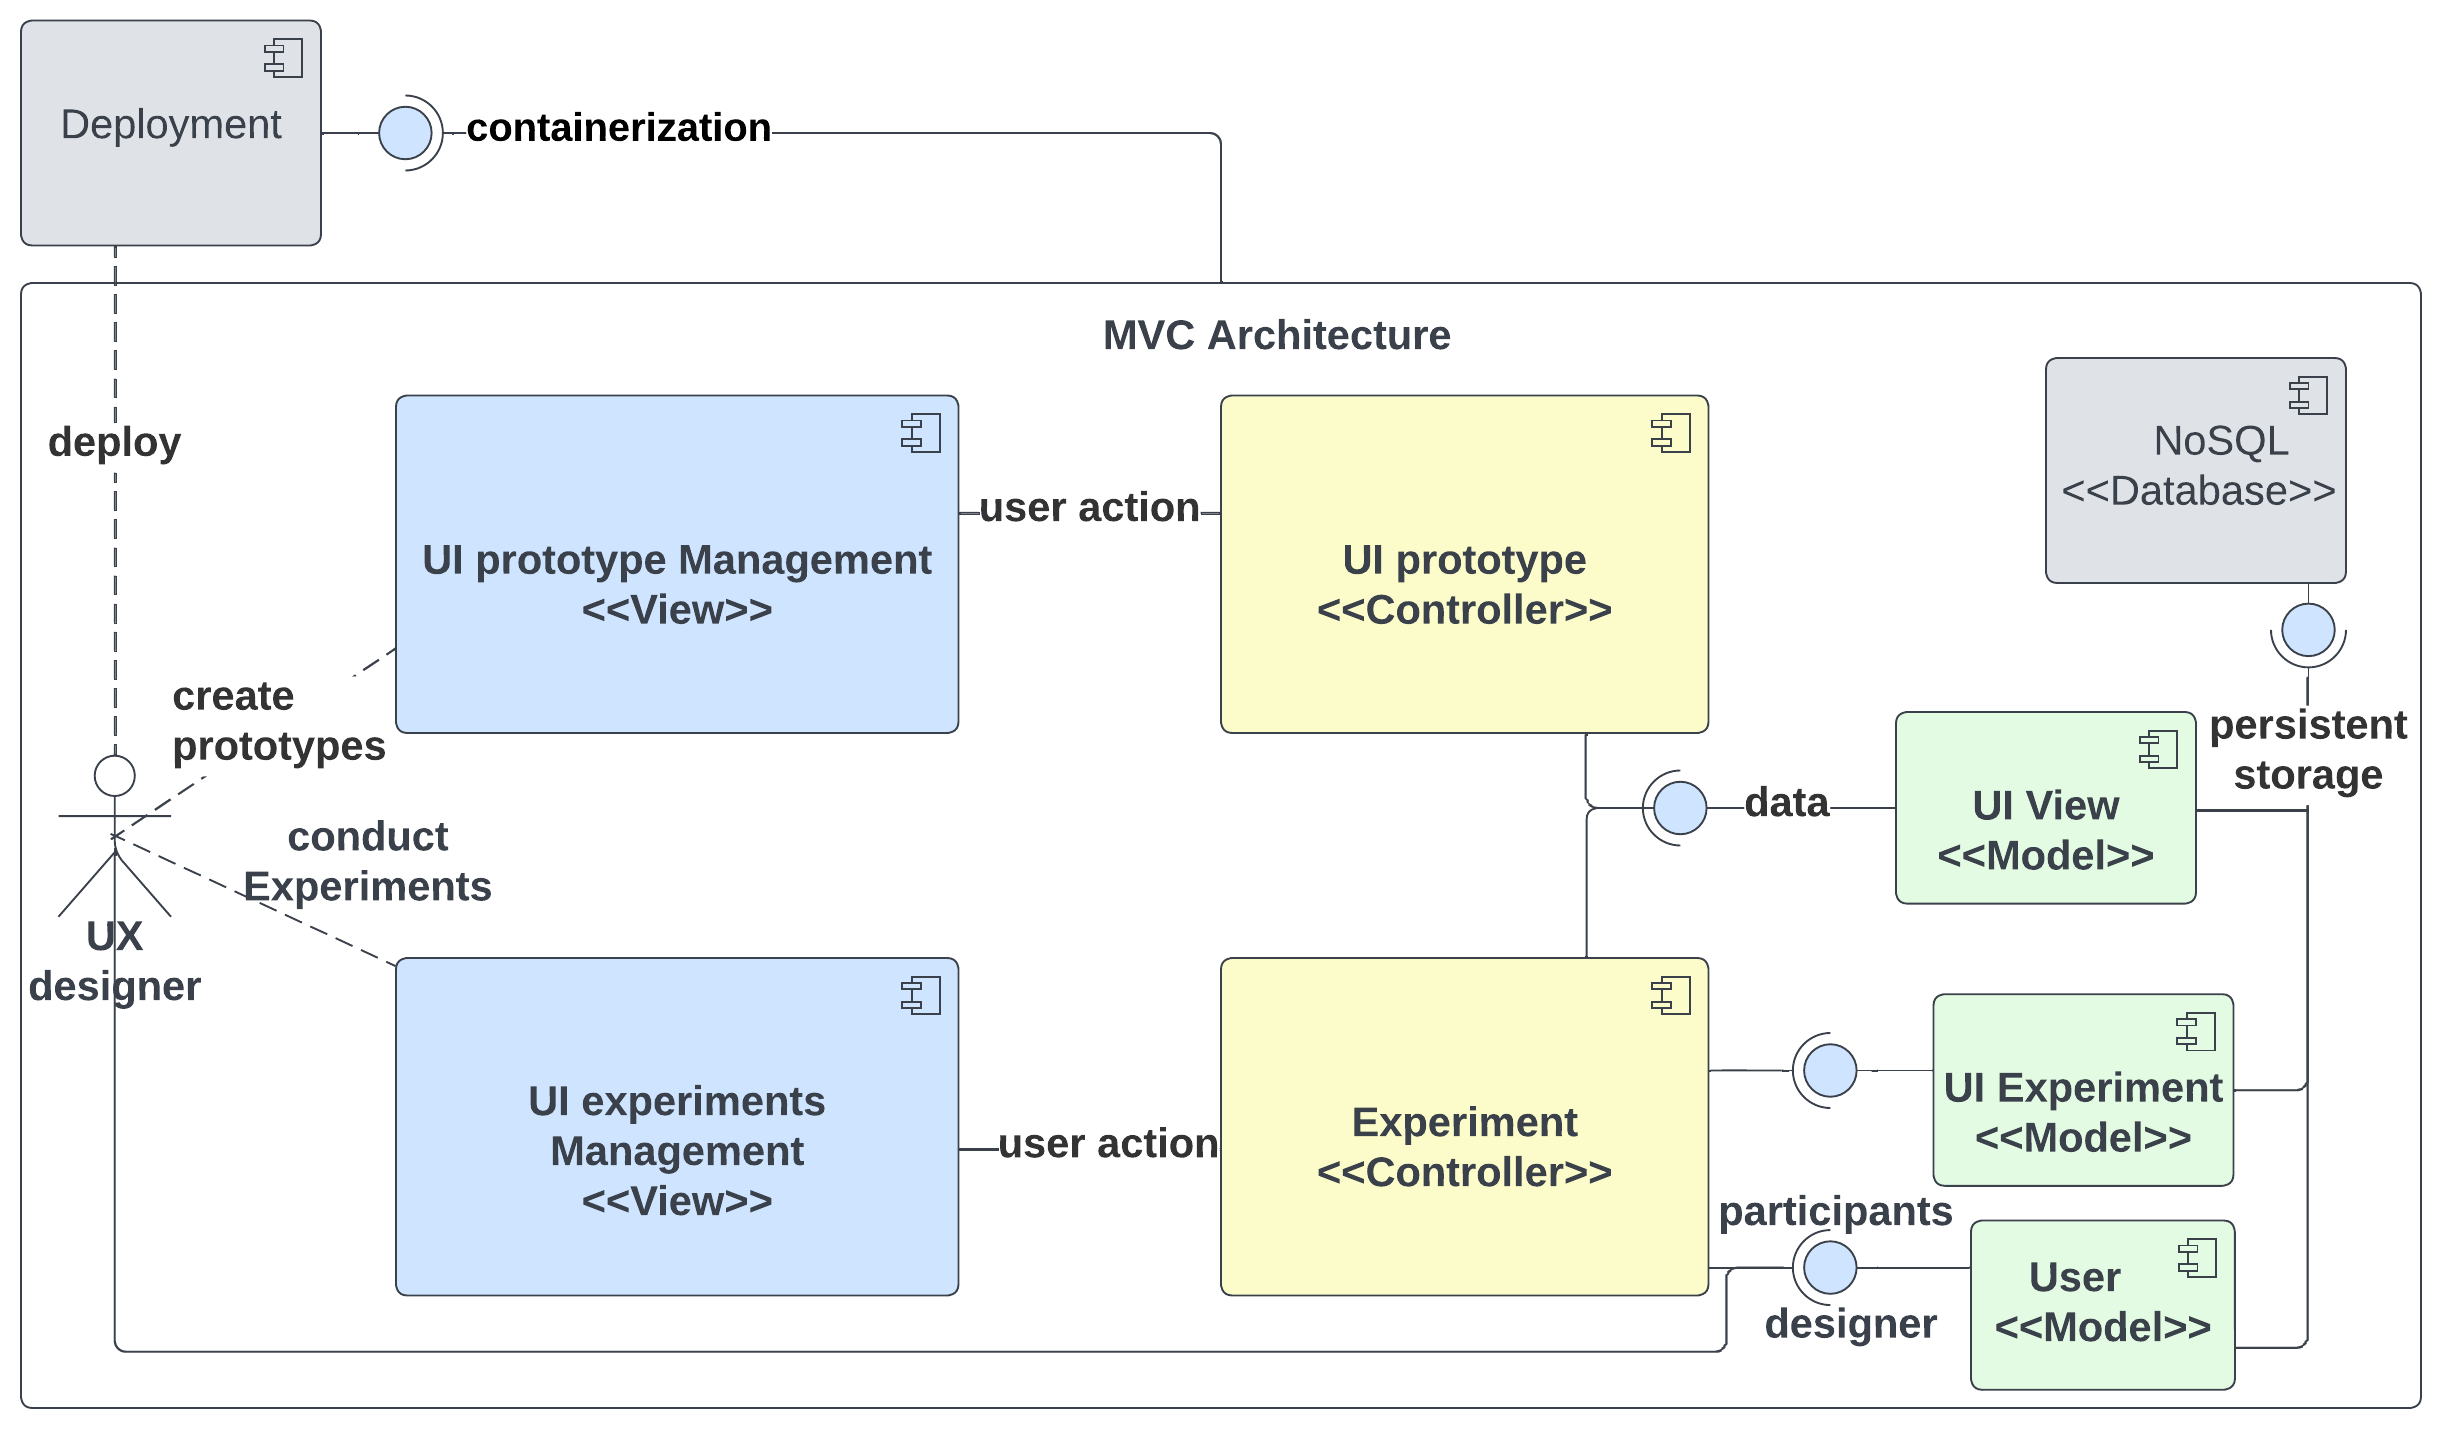
\includegraphics[width=0.9\textwidth]{MVC.png} 
    \caption[MVC Architecture of System]{MVC Architecture of our UI Prototyping tool}
    \label{fig:sc:componentD}
\end{figure}
The diagram (see figure \ref{fig:sc:componentD}) shows the different modules and components of the \ac{ui} prototyping tool and how they interact with each other during the execution of the tool.
We chose the \ac{mvc} architecture for this tool because it separates the application logic into three interconnected components. 
The model component represents the data and the business logic of the application. 
The view component represents the application's \ac{ui}, and the controller component handles the user input and updates the model and the view. 
The separation of these components allows for easier application maintenance, scalability, and modifiability.

As shown in figure \ref{fig:sc:componentD}, the \textit{UI prototype management} and the \textit{UI experiments management} are the two main views of the tool.
The \textit{UI prototype management} view manages the prototyping process, while the \textit{UI experiments management} view manages split tests and task-based usability tests. 
The \textit{UI View} model is connected to the prototyping view, and the \textit{UI experiment} model is used for split tests. 
The \textit{UI prototyping} and \textit{Experiment} controllers are the main controllers for handling user input and updating the models and views accordingly.
For the database, we use a NoSQL database that provides flexibility and scalability for applications with changing data requirements. 

The \textit{admin} user is responsible for prototyping and creating user experiments and scenarios. 
The \textit{admin} user can access all the tool's features and create, edit, and delete prototypes and experiments.
Finally, for deployment, we have one component that includes all the files and dependencies required to run the application. 
This component contains the server-side code, the client-side code, and the necessary libraries and dependencies. 
The deployment component is responsible for packaging the application and deploying it to the target environment.

In summary, the software architecture for our \ac{ui} prototyping tool is designed using the \ac{mvc} architecture, with the details explained in the next sections. 
Similarly, the role of the \textit{admin}, the user responsible for prototyping and creating user experiments and scenarios, is also explained in the next section in detail.

\clearpage
\section{UI Prototype Management}
\label{sc:section:prototyping}
In our solution approach, we must have features for creating various \ac{ui} prototypes.
Therefore, using this component, we allow the admin users to create \ac{ui} prototypes as shown in the figure \ref{fig:sc:prototyping}.
It consists of various sub-components for constructing UI elements, data models, and analyzing results.
\begin{figure}[htbp!]
    \centering    
    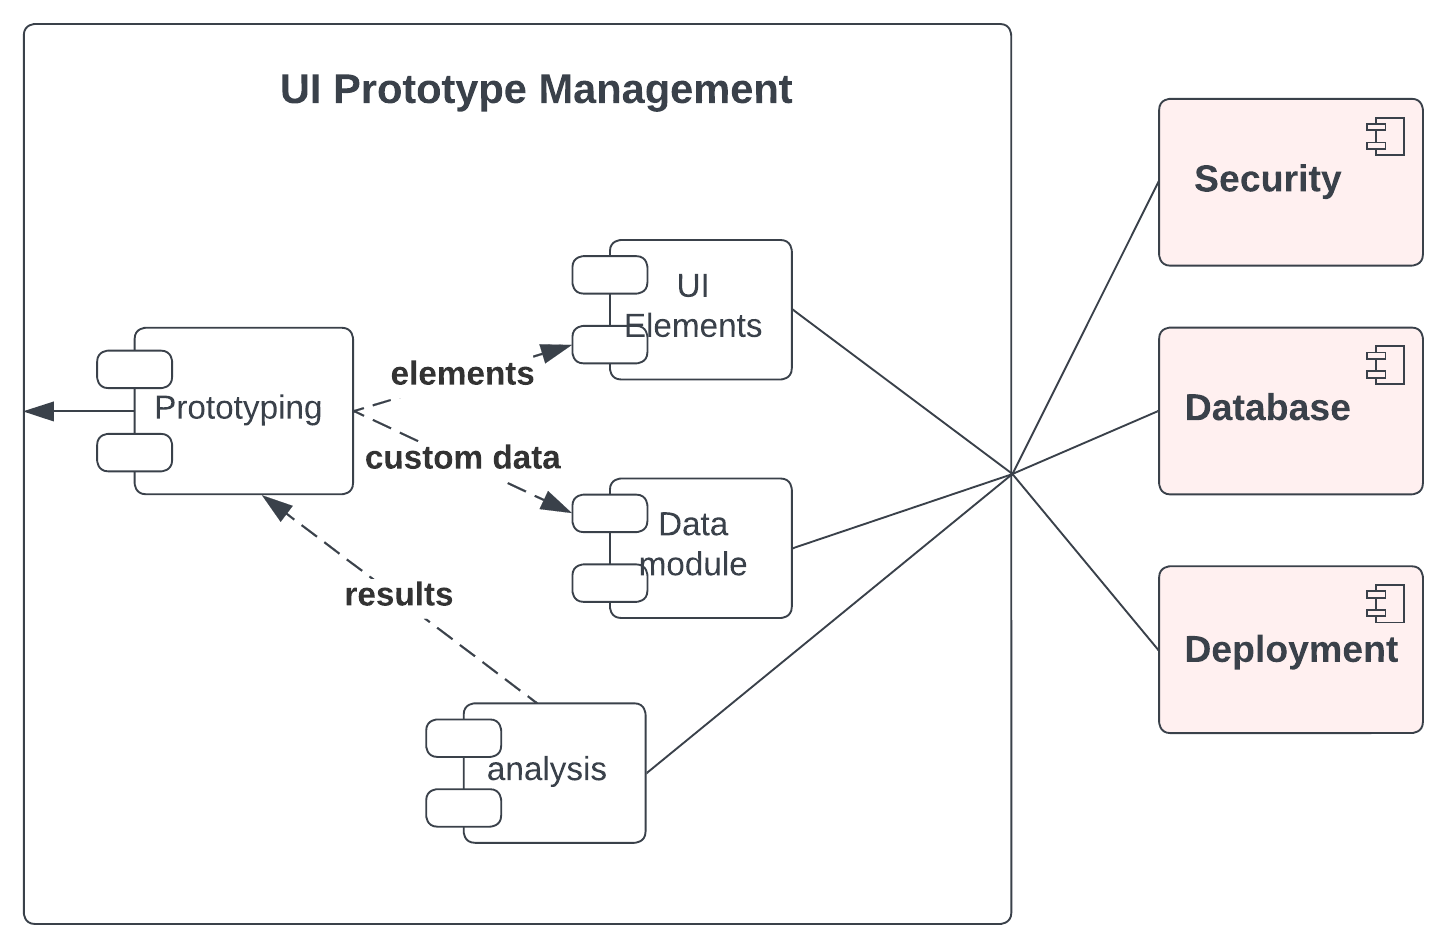
\includegraphics[width=0.9\textwidth]{UI_Prototyping.png} 
    \caption[Details of UI Prototyping Management]{Details of UI Prototyping Management connecting to a Database}
    \label{fig:sc:prototyping}
\end{figure}

\paragraph{UI Elements}
The prototype management features a comprehensive set of UI elements designed to be reusable and easy to customize. 
The UI Elements component represents various predefined UI elements used during the prototyping. 
These components can be added to a screen using a simple drag-and-drop interface, allowing users to create interactive prototypes with minimal effort quickly.
Each of our UI elements includes a range of properties that can be customized to meet the user's specific needs. 
These properties include size, color, font, and behavior properties. 
Providing these options allows users to create prototypes that accurately represent their vision without being limited by the tool's capabilities.
Some UI elements we have developed include buttons, select elements, text boxes, image render, and the input element. 
Each component is designed to be intuitive and easy to use while providing enough functionality to allow users to create complex interactions. 
\paragraph{Data Models}
The prototype management includes a data model component allowing users to create and manage data sets for their prototypes easily. 
With this component, users can create data models, which are then stored in a database and can be accessed and manipulated using a model.
Creating a data model is straightforward: users import the \ac{csv} file and then create a model for the particular data set they want to use in their prototype. 
Once the model is created, users can iterate through the data in various forms, such as a table or a grid, and visualize how the data will be displayed in their final product.
One of the key benefits of our data model component is how easily it can be modified and updated. 
Users can change the data directly within the model using a table, allowing them to quickly iterate on their prototypes without constantly importing new data sets. 
This makes it easy to test different scenarios and refine the user experience.
Similarly, by importing real-world data sets, users can create prototypes that more closely resemble the final product, which can be valuable for testing and validation.

\paragraph{Analysis}
The prototype management includes an analysis component that enables users to combine and aggregate the results of qualitative and quantitative analyses. 
By combining these different types of research, users can gain a more comprehensive understanding of how their prototype is performing and make data-driven decisions about how to iterate and improve it. 
One of the key features of our analysis component is its ability to transfer the results of the winner variant back to the prototyping component. 
It allows users to quickly iterate on their designs based on the insights gained from the analysis, ensuring that the final product is optimized for user engagement and satisfaction.\\\\
In summary, implementing a prototyping management component simplifies the \ac{ui} prototyping, helps improve the effectiveness of the UI, allowing to add \ac{ui} elements, and data models and improves the prototype.

\clearpage
\section{UI Experimentation management}
\label{sc:section:experimentation}
In our solution approach, we must have features for creating various \ac{ui} variants and conducting experiments of A/B testing. 
Therefore, as shown in figure \ref{fig:sc:experiments}, using this component, we allow the admin users to create experiments on the UI as defined in the UI prototype.
It consists of various sub-components for constructing UI variants, assigning participants to experiments, managing participants' tasks, including qualitative questions, and collecting quantitative feedback.

\begin{figure}[htbp!]
    \centering    
    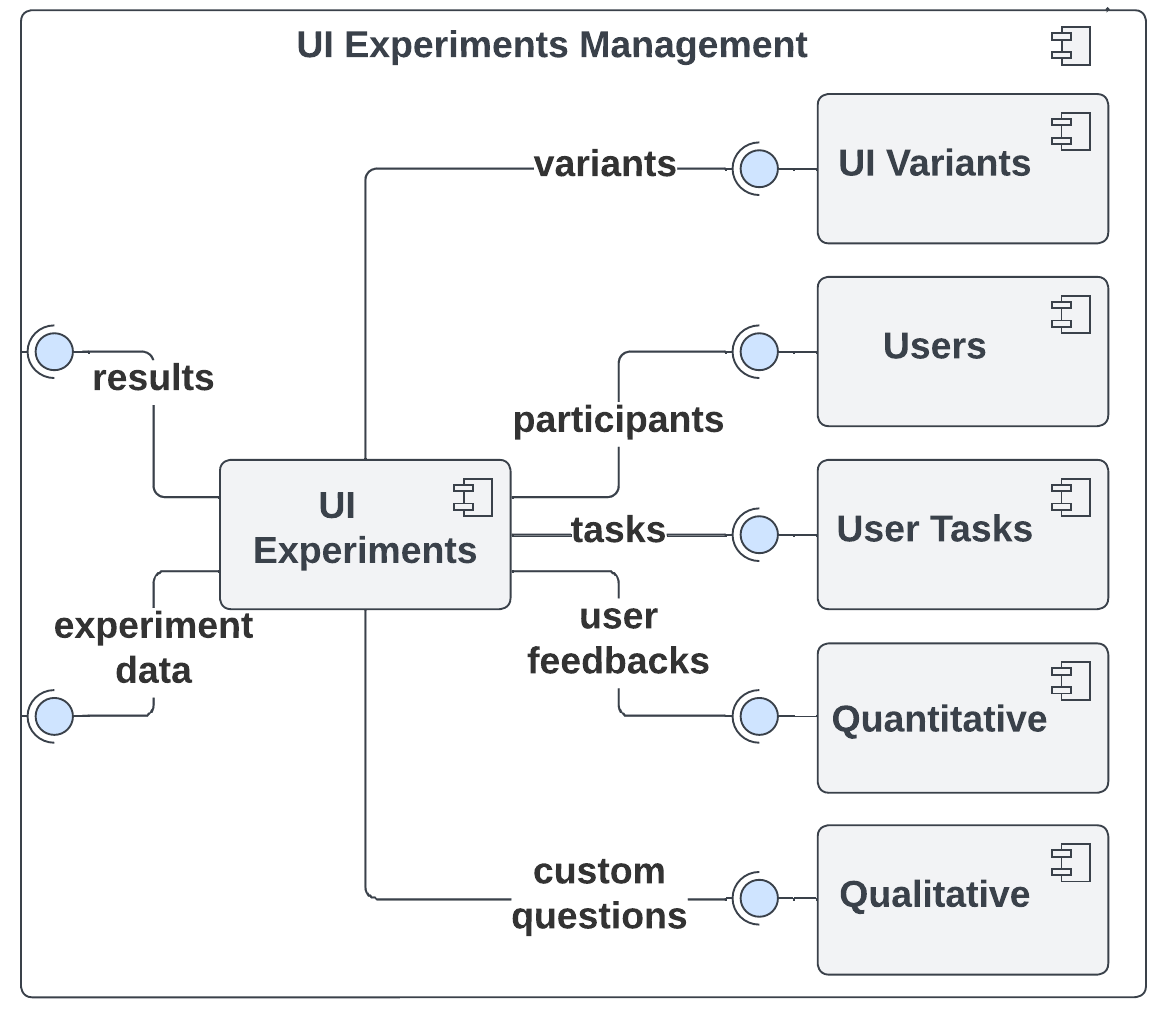
\includegraphics[width=0.9\textwidth]{UI_experiment.png} 
    \caption[Details of UI Experiment Management]{Details of UI Experiment Management connecting to a Database}
    \label{fig:sc:experiments}
\end{figure}

\paragraph{Constructing UI Variants}
The UI Variants component represents the different variations of a \ac{ui} that are used in A/B testing. 
Here, we compare two or more UI variations or variants to determine which performs better regarding user engagement and conversion rates. 
Firstly, the admin user is responsible for creating an experiment and its other variants. 
Then we modify the UI prototype for each variant to have some differences and uniqueness. 
Hence, using our interactive prototyping tool, the admin user should be able to design each variant accurately.
In the end, we have a unique prototype for each \ac{ui} variant.

\paragraph{Participants Assignments}
An important aspect while experimenting or A/B Testing is the users' participation. 
The admin user is responsible for assigning the participants to their variants. 
Therefore, we need to specify the percentage of participants allocated to an experiment variant during an experiment. 
For our solution approach, we use the between-group study such that different participants test each UI variant so that each person is only exposed to a single variant. 

\paragraph{Task Management}
We need to assign them certain user tasks to get quantitative feedback from the participants. 
It means the admin user must create certain tasks before the start of the experiment.
Our solution approach has a \textit{Tasks} component that provides a feature for creating user tasks for every UI experiment. 
These tasks are built and maintained in our tool by the admin user and are useful while collecting user feedback. 
So, the participants carry out the tasks, and our tool would collect their interaction details (e.g., time taken to finish the task, the path taken by the participant, number of unsuccessful attempts). 

\paragraph{Qualitative Questions}
The experiment management includes a qualitative component that allows users to gather participant feedback through a qualitative questionnaire. 
This component complements the quantitative component and provides users with a more holistic view of how users interact with their prototype.
The qualitative questionnaire can be easily added to the prototype, and users can choose from various question types, including open-ended and scale-based questions. 
It allows users to gather rich and detailed feedback from participants about their experience with the prototype.

\paragraph{Quantitative analysis}
The experiment management includes a quantitative component that allows users to collect data from user tasks, such as user clicks, user paths, and time taken. 
By gathering this data, users can better understand how users interact with their prototypes and identify areas for improvement.
Once the data has been gathered, the quantitative component calculates the mean for each metric. It provides users with an average value that they can use to compare different variations of their prototype and identify which one performs the best.
Users can make data-driven decisions about their prototype using the mean and quickly iterate based on user feedback. 

\paragraph{Analyze Results}
Every experiment needs to visualize its results, and the visualization component is responsible for providing this feature of analyzing the results of the A/B testing to determine which UI variant performs better. 
This component compares the user engagement and conversion rates for each variant (e.g., time to finish the task, unsuccessful attempts, etc.) and identifies the factors contributing to the performance differences. 
Once we receive the details of the winner variant from this component, the tool sends these details to the original UI prototyping management to iterate and refine the UI variants based on the experiment's results. \\\\
In summary, implementing an experiments management component simplifies the A/B testing, helps improve the effectiveness of the UI, and allows you to manage and track the different interface variations.

\clearpage
\section{Persistance}
\label{sc:section:persistance}
In our solution approach, we must have features for persisting the data in our database.
Therefore, as shown in figure \ref{fig:sc:database}, using this component, we store the data from the models from our \ac{mvc} architecture.
It consists of a \textit{Persistance infrastructure} for providing various features like \textit{database connection}, and \textit{data persistance}.

\begin{figure}[htbp!]
    \centering    
    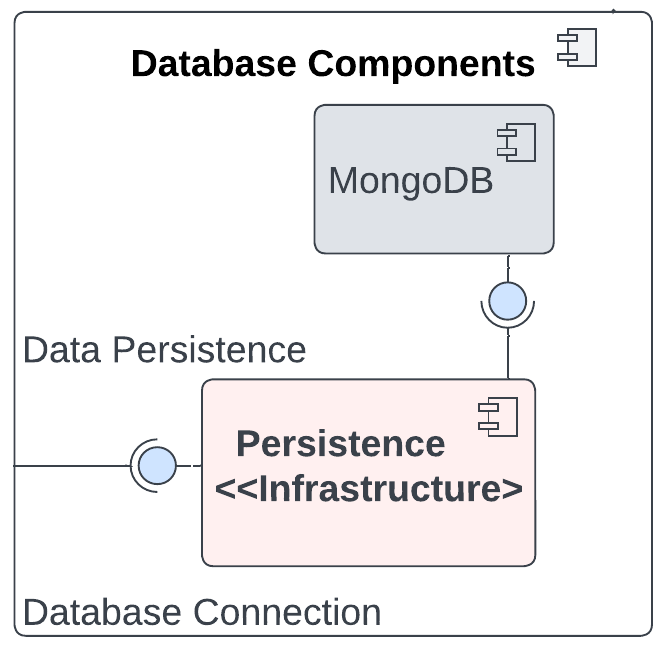
\includegraphics[width=0.6\textwidth]{Database.png} 
    \caption[Details of Database management]{Details of Database Management}
    \label{fig:sc:database}
\end{figure}

\paragraph{Persistence infrastructure}
A persistence infrastructure is necessary for our software to manage a system's data storage and retrieval. 
When a model needs to store data for later use or retrieve data that has been previously stored, a persistence infrastructure can provide the necessary functionality to accomplish this.

\paragraph{Database connection}
Our persistence infrastructure provides database connectivity for a non-relational database by using a MongoDB driver or library to interact with the database. 
We install and configure MongoDB on the appropriate servers or cloud-based environments\footnote{Cloud-based environment: \url{https://cloud.mongodb.com/}}.
Then we select a proper driver or library, configure the connection details, and use the driver or library to interact with the database in the components of the system\footnote{How to connect to cloud-based deployed MongoDB instance: \url{https://www.mongodb.com/docs/atlas/connect-to-database-deployment/}}.
Utilizing the driver or library, we interact with the non-relational database in the components of the system. It typically involves defining data models, creating, reading, updating, and deleting documents or records, and querying the database using the appropriate syntax and commands.

\paragraph{Data persistance}
After setting up the necessary drivers or libraries to connect to the MongoDB instance from the components in the system, we define the necessary CRUD (create, read, update, delete) operations for the data models.
These include methods for inserting, updating, deleting, and retrieving data from the database. 
It also provides the necessary validation and error handling for the data models and CRUD operations.\\\\
In summary, when implementing a persistence infrastructure for a non-relational database like MongoDB, we developed the structure and functionality of the database and designed the persistence layer accordingly. 
Therefore, the system can store and retrieve data in an efficient, scalable, and reliable way.

\clearpage
\section{Deployment Infrastructure}
\label{sc:section:deployment}
A deployment infrastructure is necessary for ensuring that the system is deployed and running in a secure, scalable, and reliable way. 
A deployment infrastructure is responsible for managing the deployment of components, ensuring that they are running on the appropriate servers or cloud-based environments, and monitoring their performance.
We use a no-code platform and microservice architecture to simplify deployment infrastructure implementation. It allows for the creation of deployment pipelines and automates many of the processes involved in deploying components.

\begin{figure}[htbp!]
    \centering    
    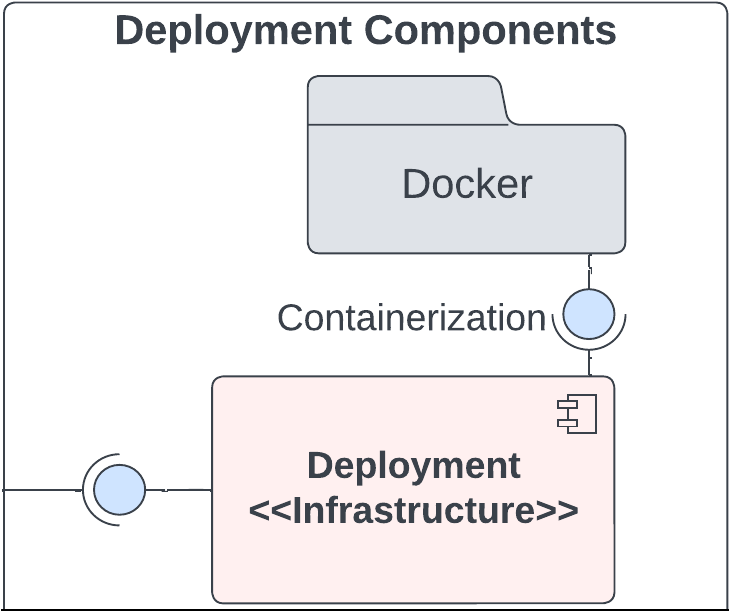
\includegraphics[width=0.6\textwidth]{Deployment.png} 
    \caption[Details of Deployment components]{Details of Deployment components}
    \label{fig:sc:deployment}
\end{figure}

\paragraph{Code Generation}
We use a no-code approach using code generation to simplify the implementation of our deployment infrastructure by automating many of the tasks involved in deploying the system.
So, we define a set of rules and templates for automatic code generation and generate some reusable components as defined by the UI prototyping management. 
These components' implementation uses templates containing its code (e.g., for a button element defined in the UI prototype, a template is generated containing all its properties and logic).
Then, the code generator takes input data, including configuration files, database schemas, and models of system components and their interactions. 
Finally, the code will be generated using the templates and rules defined in the previous steps, and we will containerize the generated code. 

\paragraph{Containerization}
Containerization plays an even more important role in using a microservice architecture. 
It must support the deployment of many independent microservices that may be deployed across multiple servers or databases.
From our component diagram, we first identify the system's microservices and their dependencies, such as database components, UI prototyping management, and UI experimentation management. 
It helps determine how the microservices should be deployed and how they should communicate.
Next, we create Docker images for each microservice and its dependencies.
Then, we define docker-compose files\footnote{A Docker Compose file is a YAML file that specifies the microservices, their dependencies, and how they should be deployed and connected.} in yaml\footnote{YAML format for files: \url{https://www.redhat.com/en/topics/automation/what-is-yaml}} (see Appendix \ref{appendix:one:installation}) that describe how the docker containers should be deployed and connected.
Finally, we build the \textit{docker images} and deploy them as \textit{docker containers}. \\\\
In summary, implementing a deployment infrastructure for a microservice architecture can simplify the deployment and management of microservices, making it easier to build and maintain complex systems.

\clearpage
\section{Security Infrastructure}
\label{sc:section:security}
Security infrastructure is essential to protect the system from unauthorized access and attacks. 
By implementing security measures, such as access control, we limit access to sensitive information and functions to only authorized users.
Similarly, authentication is one of the fundamental security mechanisms used to verify the identity of users.
Our security infrastructure, therefore, provides access control and some authentication mechanisms.

\begin{figure}[htbp!]
    \centering    
    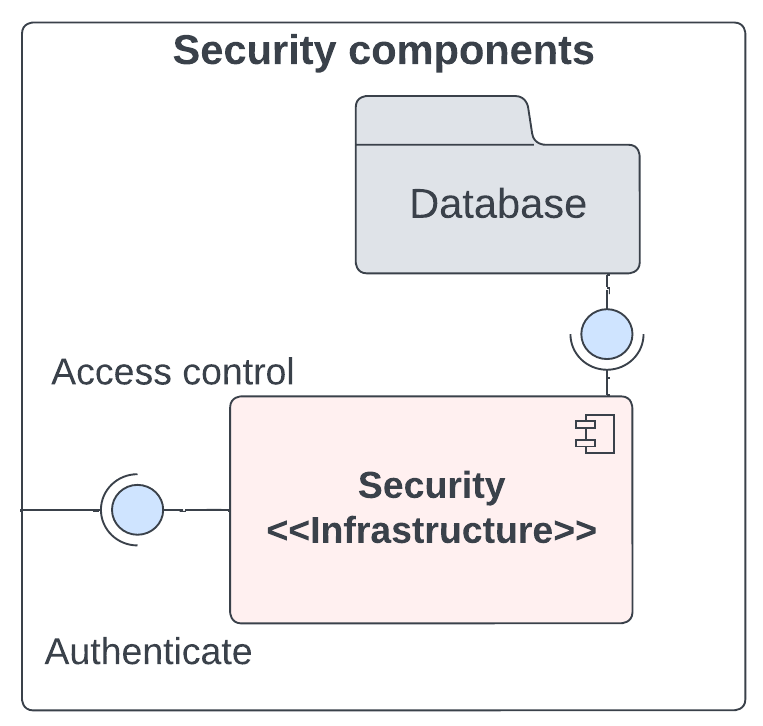
\includegraphics[width=0.6\textwidth]{Security.png} 
    \caption[Details of Security components]{Details of Security components}
    \label{fig:sc:security}
\end{figure}

\paragraph{Access control}
Access control involves defining policies and rules determining who can access resources under what circumstances.
Therefore we implement access control mechanisms using role-based access control (RBAC) and then allowing or denying access based on those roles or groups.
So, we first identify the roles or groups requiring system access, including participants, administrators, and other users\footnote{This may include different stakeholders like designers, product managers, developers, etc.}. 
Then we define the access rights (e.g., the UI prototyping management should only be accessible to the admin users).
Finally, we implement a mechanism that checks the user roles and then accesses the data or services accordingly. 

\paragraph{Authentication mechanisms}
Authentication involves verifying the identity of users and ensuring that they have the appropriate permissions to access the system.
We provide an authentication mechanism using a password and username. 
It ensures that only authorized users can access our tool.
Moreover, we define some validators for password strength to make sure the passwords are strong.\\\\
In summary, implementing a security infrastructure providing access control and authentication mechanisms for our tool can help prevent unauthorized access and protect sensitive data from being compromised.

\clearpage